\chapter{Hasil dan Analisis} 

\section{Prelude: Pemilihan Training Data}

Perlu diperhatikan bahwa pada kasus ini, anomaly detection dikembangkan dengan pendekatan \emph{unsupervised learning}. Hal ini karena data \texttt{machine\textunderscore status} tidak mewakili apakah data berupa anomaly atau tidak.Ingat bahwa permasalahan yang ingin diselesaikan disini adalah mencari pola pada data yang mengindikasi penyebab kerusakan mesin. Hal ini berarti anomaly yang ingin dideteksi terjadi sebelum status mesin \texttt{BROKEN}. 

Data pada bulan 8 dipilih sebagai training data karena pada bulan tersebut tidak terjadi kerusakan mesin. Disini penulis berasumsi bahwa pada bulan 8 tidak terjadi anomali sama sekali pada data, karena tidak terjadi kerusakan mesin. Namun pada bulan lainnya, walau ada bagian data yang memiliki status mesin NORMAL, bisa saja sebenarnya sudah terjadi anomaly yang menyebabkan machine BROKEN pada hari-hari setelahnya.

\section{Hasil}
\subsection{LSTM Autoencoder}

Data dipisah menjadi dua bagian, yaitu data normal yang mengandung data dari status NORMAL dan data anomali yang berasal dari status selain NORMAL (BROKEN dan RECOVERY).

Kemudian data dibagi menjadi 3 dataset, yaitu train, validation, dan test. Data train dan validation diambil pada bulan ke-8 awal dan akhir masing-masing dan digunakan untuk training model, sedangkan data test diambil pada selain bulan ke-8 untuk memprediksi hasil anomali.

Proses training model LSTM Autoencoder dilakukan sebanyak 5 epoch dengan menggunakan GPU (CUDA). Analisis dibagi menjadi dua macam, yaitu dengan PCA dan tanpa PCA.

Kemudian dilakukan prediksi pada data test dari model yang telah dilakukan training sehingga dapat diperoleh nilai loss yang dihasilkan.

    \subsubsection{Dengan PCA}

    \begin{figure}[h]
        \centering
        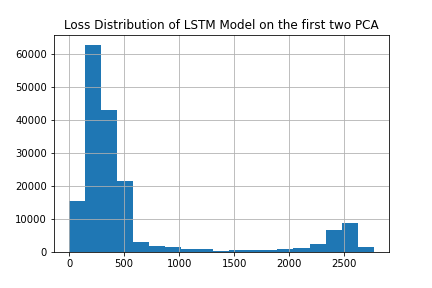
\includegraphics[width=0.6\textwidth]{resources/LSTM/LSTM_PCA_LossDist.png}
        \caption{Distribusi loss LSTM dengan PCA}
    \end{figure}

    \begin{figure}[h]
        % \centering
        \centerline{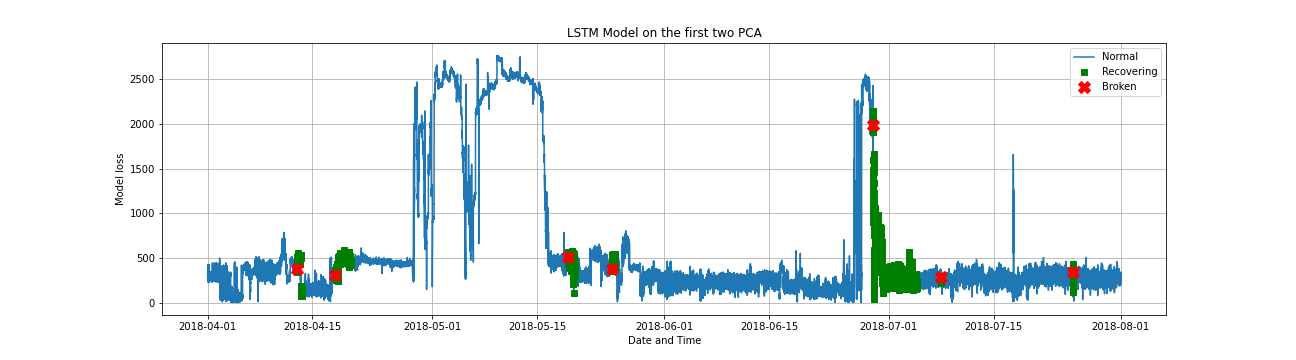
\includegraphics[width=1.4\textwidth]{resources/LSTM/LSTM_PCA_model_loss.png}}
        \caption{Plot loss LSTM dengan PCA}
    \end{figure}

    Dengan menggunakan nilai threshold 500, diperoleh jumlah data anomali sebagai berikut.

    \begin{table}[h]
        \centering
        \begin{tabular}{|l|r|r|r|}
            \hline
            \multicolumn{1}{|c|}{\textbf{Jenis anomali}} & \multicolumn{1}{c|}{\textbf{Jumlah}} & \multicolumn{1}{c|}{\textbf{Total data}} & \multicolumn{1}{c|}{\textbf{Persentase (\%)}} \\ \hline
            Anomali pada data NORMAL                     & 33.866                                & 160.430                                   & 21                                       \\ \hline
            Anomali pada data selain NORMAL              & 2.237                                 & 14.454                                    & 15                                       \\ \hline
        \end{tabular}
    \end{table}

    Jumlah anomali pada data selain NORMAL tidak mencakup keseluruhan total data sehingga terdapat prediksi yang berada pada data dalam kondisi BROKEN atau RECOVERY.

    \subsubsection{Tanpa PCA}

    \begin{figure}[h]
        \centering
        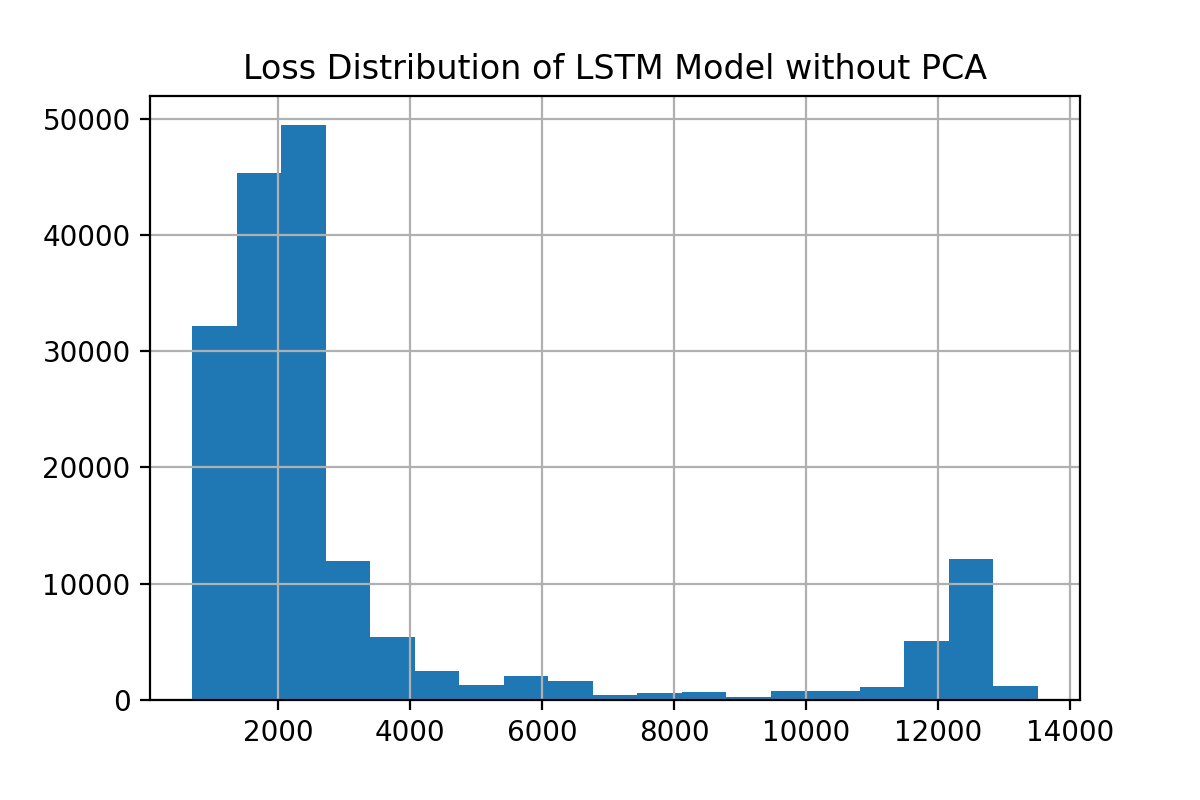
\includegraphics[width=0.6\textwidth]{resources/LSTM/LSTM_noPCA_LossDist.png}
        \caption{Distribusi loss LSTM tanpa PCA}
    \end{figure}

    \begin{figure}[h]
        % \centering
        \centerline{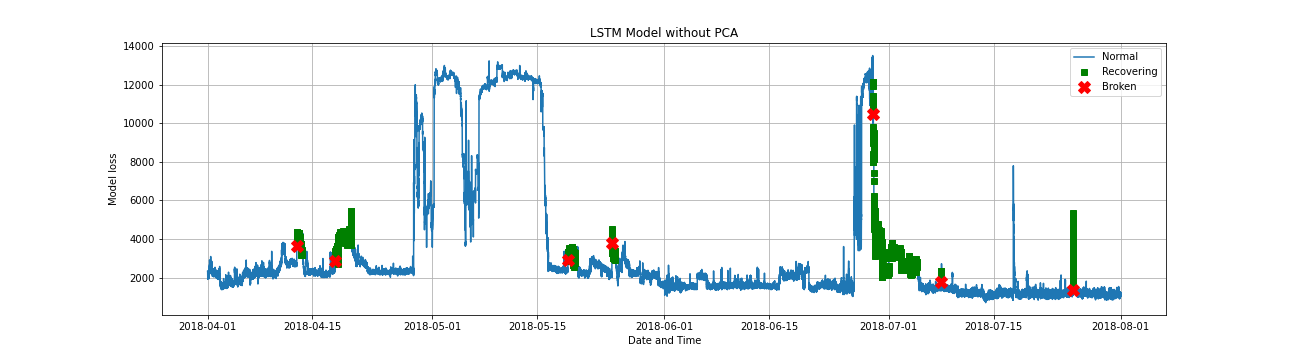
\includegraphics[width=1.4\textwidth]{resources/LSTM/LSTM_noPCA_model_loss.png}}
        \caption{Plot loss LSTM tanpa PCA}
    \end{figure}

    Dengan menggunakan nilai threshold 3500, diperoleh jumlah data anomali sebagai berikut.

    \begin{table}[h]
        \centering
        \begin{tabular}{|l|r|r|r|}
            \hline
            \multicolumn{1}{|c|}{\textbf{Jenis anomali}} & \multicolumn{1}{c|}{\textbf{Jumlah}} & \multicolumn{1}{c|}{\textbf{Total data}} & \multicolumn{1}{c|}{\textbf{Persentase (\%)}} \\ \hline
            Anomali pada data NORMAL                     & 30.182                                & 160.430                                   & 19                                       \\ \hline
            Anomali pada data selain NORMAL              & 4.979                                 & 14.454                                    & 34                                       \\ \hline
        \end{tabular}
    \end{table}

    Terlihat bahwa jumlah anomali pada data NORMAL lebih sedikit 3\% dari analisis dengan PCA, Namun jumlah anomali pada data selain NORMAL juga meningkat hampir 2 kali lipat.

\subsection{Bayesian Probability}

Data dipisah menjadi training data dan test data. Tidak ada validation data disini, karena validation data digunakan untuk mencegah model overfitting pada training data. Namun karena model bayesian adalah distribusi probabilitas, maka validation data akan menggeser kontur probabilitas dari overfitting pada training data menjadi tepat fit pada training dan validation data sekaligus. Jadi hasilnya tidak akan ada bedanya jika model dilatih pada training dan validation data yang digabungkan. Karena itu, validation data sudah digabungkan kedalam training data, yaitu data pada bulan 8.

Hasil prediksi model Bayesian pada test data menghasilkan distribusi probabilitas data merupakan data normal diperoleh pada \ref{bayes_probdist}. Kemudian probabilitas tidak terjadi anomali dan terjadi anomali pada tiap waktu diperoleh pada \ref{bayes_normal_pmf} dan \ref{bayes_anomaly_pmf}. Perlu diperhatikan bahwa \ref{bayes_anomaly_pmf} hanyalah $ 1 - P(x_n) $ dari tiap data pada \ref{bayes_normal_pmf}, namun grafik probabilitas anomaly lebih mudah untuk dikomparasikan dengan hasil grafik model loss pada metode LSTM Autoencoder.

\begin{figure}[H]
    \centering
    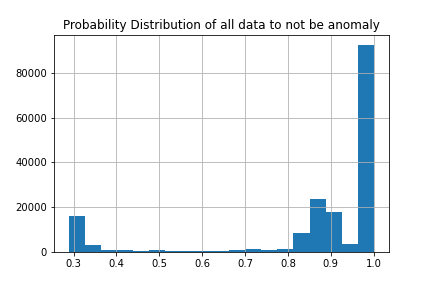
\includegraphics[width=0.8\textwidth]{resources/Bayes/Bayes_ProbDist.png}
    \caption{Prediksi Probabilitas bukan Anomali} \label{bayes_probdist}
\end{figure}
\begin{figure}[H]
    %\centering
    \centerline{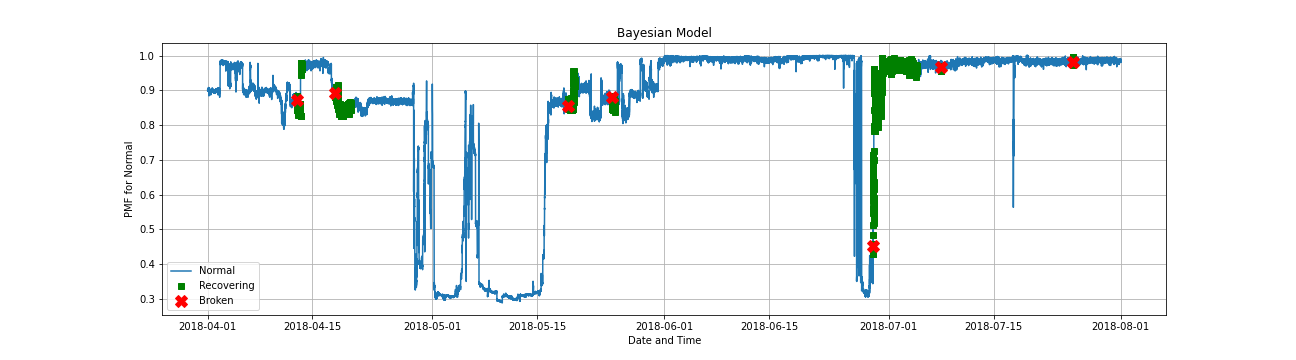
\includegraphics[width=1.4\textwidth]{resources/Bayes/Bayes_normal_PMF.png}}
    \caption{Prediksi Probabilitas bukan Anomali} \label{bayes_normal_pmf}
\end{figure}
\begin{figure}[H]
    %\centering
    \centerline{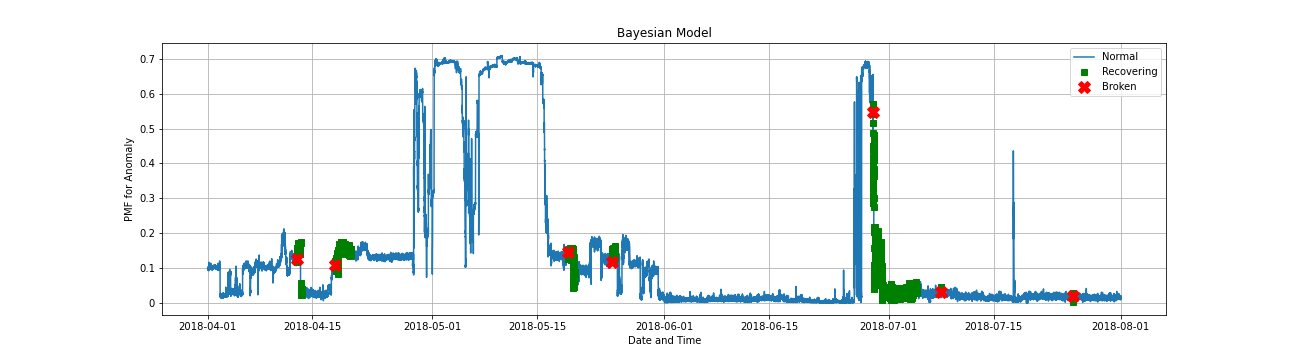
\includegraphics[width=1.4\textwidth]{resources/Bayes/Bayes_anomaly_PMF.png}}
    \caption{Prediksi Probabilitas terjadi Anomali} \label{bayes_anomaly_pmf}
\end{figure}

Dengan menetapkan nilai threshold sebesar 0.85, ini berarti jika probabilitas suatu data merupakan data normal dibawah 0.85 sudah ditetapkan sebagai data yang likely merupakan anomaly. Diperoleh jumlah data anomali sebagai berikut.

\begin{table}[h]
    \centering
    \begin{tabular}{|l|r|r|r|}
        \hline
        \multicolumn{1}{|c|}{\textbf{Jenis anomali}} & \multicolumn{1}{c|}{\textbf{Jumlah}} & \multicolumn{1}{c|}{\textbf{Total data}} & \multicolumn{1}{c|}{\textbf{Persentase (\%)}} \\ \hline
        Anomali pada data NORMAL                     & 34.527                                & 160.430                                   & 22                                       \\ \hline
        Anomali pada data selain NORMAL              & 2.567                                 & 14.454                                    & 18                                       \\ \hline
    \end{tabular}
\end{table}

\section{Analisis} \label{ANALISIS}
\subsection{Komparasi Kecepatan Proses}
Kecepatan proses yang diukur adalah durasi waktu yang dibutuhkan untuk model training. Didapatkan hasil berikut.

\begin{table}[h]
    \centering
    \begin{tabular}{|l|r|l|}
        \hline
        \multicolumn{1}{|c|}{\textbf{Model}} & \multicolumn{1}{c|}{\textbf{Durasi Model Training}} & \multicolumn{1}{c|}{\textbf{Keterangan}} \\ \hline
        Interquartile Range (IQR)   & 1s 100ms 176$\mu$s      & Acuan     \\ \hline
        K-Means Clustering          & 46s 063ms 282$\mu$s     & Acuan     \\ \hline
        Isolation Forest            & 15s 139ms 811$\mu$s     & Acuan     \\ \hline
        Bayesian Probability        & 15s 031ms 475$\mu$s     & Kembangan \\ \hline
        LSTM Autoencoder dengan PCA & 18m 02s 607ms 847$\mu$s & Kembangan \\ \hline
        LSTM Autoencoder tanpa PCA  & 39m 20s 885ms 569$\mu$s & Kembangan \\ \hline
    \end{tabular}
\end{table}

Terlihat bahwa durasi model training cukup cepat, kecuali untuk model LSTM Autoencoder. Hal ini karena LSTM Autoencoder memiliki basis Neural Network yang mempunyai multilayer. Dalam model yang penulis kembangkan, total layer sebanyak 128 lapis, yang membuat proses komputasi cukup ekstensif walau sudah dibantu dengan menggunakan driver CUDA.

Model IQR dan Bayesian membutuhkan durasi yang cukup sedikit. Hal ini karena model dilatih dengan perhitungan statistik yang sederhana secara komputasi. Model IQR hanya perlu menghitung tiap data terhadap range antar quartil atas dan quartil bawah. Kemudian model Bayesian sudah menggunakan penyederhanaan matematik secara analitik yang cukup panjang, sehingga iterasi numerik yang perlu dilakukan tidak terlalu kompleks. Hal ini juga dibantu dengan scale down data input pada model Bayesian. Walaupun model Bayesian yang menggunakan matematik yang jauh lebih rumit dibandingkan IQR membuat durasi training 15x lebih lama.

Model K-Means Clustering dan Isolation Forest memakan durasi yang kecil karena pendekatan yang dilakukan adalah menganggap data hanya terbagi antara 2 kluster saja, yaitu kluster normal dan anomaly. Apabila asumsi kluster lebih dari 2 mungkin akan memakan waktu lebih lama, namun ini sudah bukan lagi Anomaly Detection melainkan Clustering Data.

    \subsection{Perbandingan Prediksi Anomali}
    Terlihat pada plot bahwa ketiga model kembangan menunjukkan hasil deteksi anomali yang cukup mirip. Karena pendekatan pengembangan data yang digunakan adalah \textit{unsupervised learning}, terdapat beberapa anomali yang muncul pada saat sebelum terjadinya kerusakan mesin yang menunjukkan bahwa walaupun status mesin pada saat itu adalah NORMAL, namun sudah ada indikasi bahwa mesin akan mengalami kerusakan beberapa waktu ke depan.

    \begin{figure}[h]
        %\centering
        \centerline{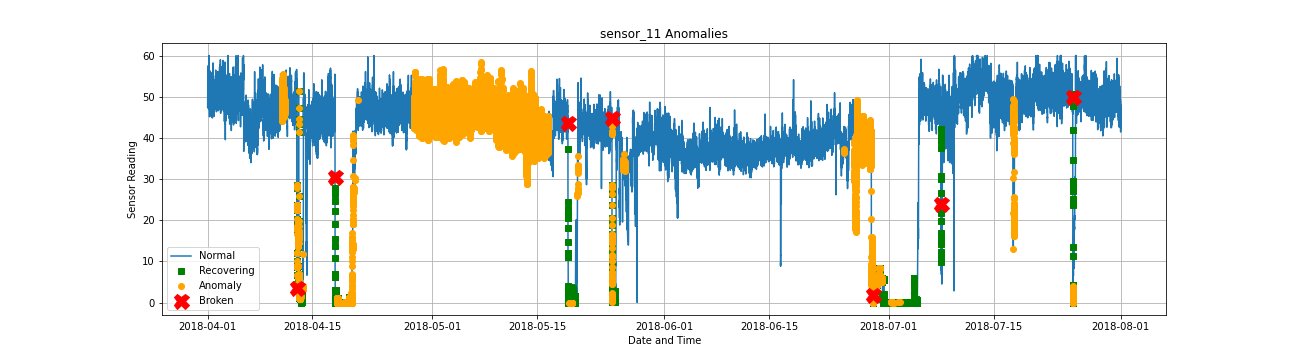
\includegraphics[width=1.4\textwidth]{resources/LSTM/LSTM_noPCA_sensor_11.png}}
        \caption{Hasil deteksi anomali model LSTM tanpa PCA}
    \end{figure}
    
    \begin{figure}[h]
        %\centering
        \centerline{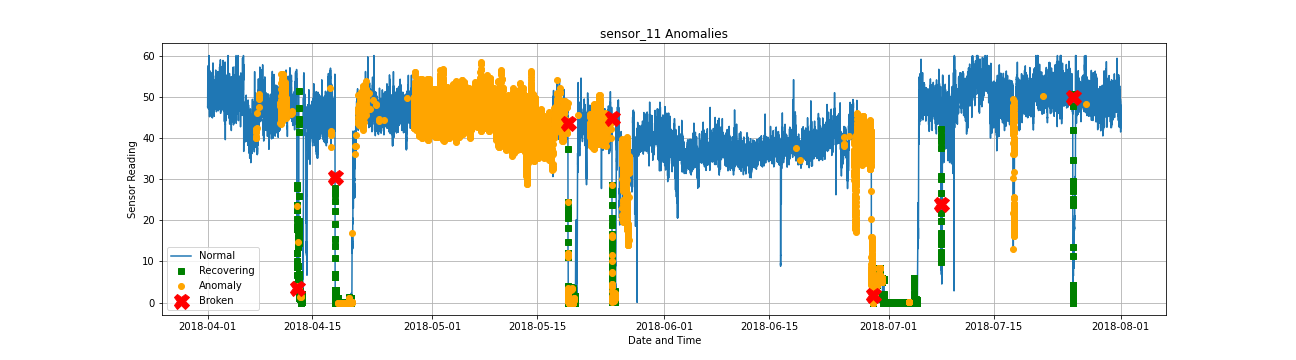
\includegraphics[width=1.4\textwidth]{resources/LSTM/LSTM_PCA_sensor_11.png}}
        \caption{Hasil deteksi anomali model LSTM dengan PCA}
    \end{figure}
    
    \begin{figure}[h]
        %\centering
        \centerline{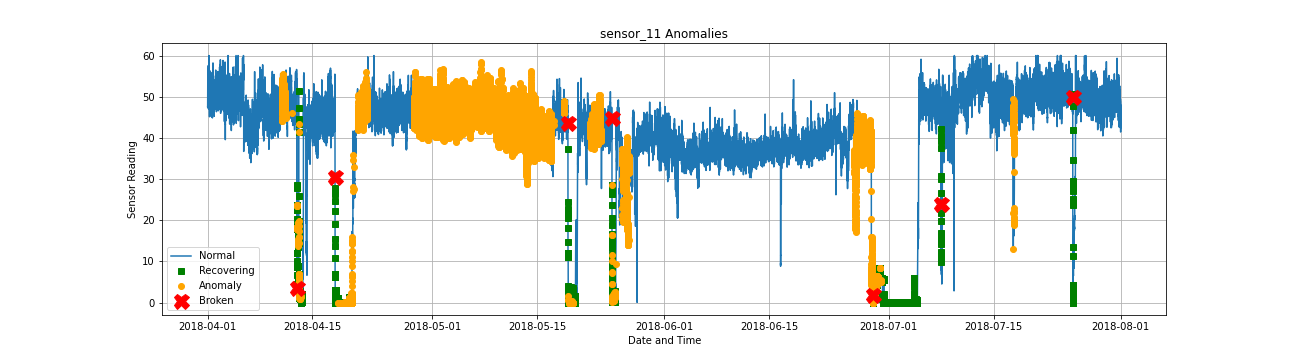
\includegraphics[width=1.4\textwidth]{resources/Bayes/Bayes_sensor_11.png}}
        \caption{Hasil deteksi anomali model Bayesian}
    \end{figure}

    Sedangkan jika dilihat dari model loss, ketiga model kembangan menunjukkan bahwa hanya terdapat satu data dengan kerusakan mesin yang memiliki nilai loss tinggi cukup tinggi. Hal ini menunjukkan bahwa anomali tidak harus terjadi pada saat terjadi kerusakan mesin, sehingga mendukung pendekatan \textit{unsupervised learning}.

    \begin{table}[H]
        \centering
        \begin{tabular}{|l|r|l|}
            \hline
            \multicolumn{1}{|c|}{\textbf{Metode}} & \multicolumn{1}{c|}{\textbf{Persentase (\%)}} & \multicolumn{1}{c|}{\textbf{Keterangan}} \\ \hline
            Interquartile Range (IQR)   & 14 & Acuan     \\ \hline
            K-Means Clustering          & 13 & Acuan     \\ \hline
            Isolation Forest            & 13 & Acuan     \\ \hline
            Bayesian Probability        & 22 & Kembangan \\ \hline
            LSTM Autoencoder dengan PCA & 21 & Kembangan \\ \hline
            LSTM Autoencoder tanpa PCA  & 19 & Kembangan \\ \hline
        \end{tabular}
    \end{table}

    Karena prediksi pada model acuan tidak menghasilkan distribusi loss dari model maka akan dianalisis berdasarkan jumlah anomali yang diprediksi. Hasil prediksi model kembangan seluruhnya menghasilkan jumlah yang lebih besar dari model acuan. Namun perbandingan jumlah prediksi dirasa kurang akurat karena bergantung oleh nilai threshold yang digunakan tiap model.

    \subsection{Keberhasilan Memprediksi Kerusakan Mesin}

    Asumsi yang digunakan adalah sebelum terjadi kerusakan mesin, akan terdeteksi anomali. Hasil pengukuran sensor yang menunjukkan data anomali ini lah yang mengindikasikan bahwa terjadi hal yang tidak wajar pada mesin dan akan menyebabkan kerusakan jika dibiarkan. Untuk melihat keberhasilan tiap model memprediksi kerusakan mesin, atau mendeteksi anomali yang menyebabkan mesin rusak, dapat dilihat lebih mudah pada grafik-grafik \ref{IQRms}, \ref{KMms}, \ref{IFms}, \ref{Bms}, \ref{nPms}, \ref{wPms}.

    Pada model acuan IQR (\ref{IQRms}), kerusakan yang terprediksi hanyalah kerusakan mesin ketiga dan kelima. Kerusakan mesin pertama terdeteksi anomali sebanyak 2x namun dengan interval waktu yang cukup jauh sehingga terbilang gagal memprediksi kerusakan pertama.

    Pada model acuan K-Means Clustering (\ref{KMms}) dan Isolation Forest (\ref{IFms}), hasil prediksi cukup mirip. Kerusakan mesin ke 3, 5, 6, dan 7 terprediksi dengan baik. Namun Isolation Forest mampu mendeteksi anomali sebelum kerusakan keempat, sehingga lebih bagus dibandingkan model K-Means Clustering.

    Model Bayesian (\ref{Bms}) cukup berbeda, kerusakan yang terprediksi adalah kerusakan ke 1, 3, 4, dan 5. Ini menarik karena kerusakan pertama berhasil terprediksi sementara ketiga model acuan gagal mendeteksi hal tersebut. Akan tetapi kerusakan ke 6 dan 7 gagal terprediksi oleh model Bayesian.

    Model LSTM lebih menarik lagi. Untuk LSTM tanpa PCA (\ref{nPms}), kerusakan yang terprediksi adalah kerusakan ke 1, 3, dan 5. Sementara LSTM dengan PCA (\ref{wPms}) berhasil memprediksi kerusakan ke 1, 2, 3, 4, dan 5. Hal ini tidak terekspektasi, karena LSTM tanpa PCA dilatih langsung dengan data 52 sensor sekaligus sementara LSTM dengan PCA hanya dilatih dengan data hasil PCA saja. Hal yang dapat disimpulkan dari fenomena ini adalah model LSTM tanpa PCA mengalami \emph{overfitting} pada data sensor. Sementara LSTM yang menggunakan PCA berhasil menangkap pola data yang penting saja, yaitu yang terkandung dalam PCA.

    Terlihat bahwa model yang berperforma paling buruk adalah model acuan IQR. Kemudian model acuan K-Means Clustering dan Isolation Forest unggul dalam memprediksi kerusakan mesin pada bulan-bulan akhir yaitu kerusakan ke 6 dan 7. Sementara model kembangan ketiganya unggul dalam mempredeksi kerusakan pada bulan-bulan awal, terutama model LSTM tanpa PCA yang berhasil mempredeksi kerusakan 5 kali secara beruntun.

    Perlu diperhatikan bahwa metode LSTM berhasil mendeteksi kerusakan kedua, yang memiliki anomali yang overlap dengan data normal. Anomali yang overlap dengan data normal ini lah yang menyebabkan kegagalan metode-metode berbasis clustering untuk mendeteksi data tersebut sebagai anomali. Namun LSTM yang berbasis Neural Network memiliki mekanisme yang sangat berbeda sehingga mampu mendeteksi anomali overlap ini.

    \subsection{The Best Model}

    Diperoleh bahwa terdapat 2 model terbaik yang mampu memprediksi kerusakan mesin terbanyak, yaitu model acuan Isolation Forest dan model kembangan LSTM Autoencoder dengan PCA. Untuk menganalisis lebih jauh, maka perlu diperhatikan hasil prediksi kerusakan yang gagal. Yaitu hasil prediksi yang menunjukkan anomali namun ternyata tidak terjadi kerusakan mesin akibat anomali tersebut. Hal ini diistilahkan sebagai \emph{false positive anomaly}.

    Terlihat seperti pada \ref{IFms} bahwa model memprediksi beberapa anomali pada akhir bulan 5 dan awal bulan 6, yang kemudian berhenti memprediksi anomali untuk interval waktu yang cukup lama. Ini menandakan bahwa model mamprediksi beberapa anomali yang \emph{false positive} pada waktu tersebut.

    Pada model LSTM Autoencoder dengan PCA (\ref{wPms}), terdapat hasil prediksi anomali yang \emph{false positive} pada akhir bulan 5, namun tidak ada anomali \emph{false positive} pada awal bulan 6. Ini berarti model LSTM Autoencoder dengan PCA memiliki \emph{false positive rate} lebih rendah dari model Isolation Forest.